\let\negmedspace\undefined
\let\negthickspace\undefined
\documentclass[journal,12pt,twocolumn]{IEEEtran}
\usepackage{cite}
\usepackage{amsmath,amssymb,amsfonts,amsthm}
\usepackage{algorithmic}
\usepackage{graphicx}

\usepackage{textcomp}
\usepackage{xcolor}
\usepackage{txfonts}
\usepackage{listings}
\usepackage{enumitem}
\usepackage{mathtools}
\usepackage{gensymb}
\usepackage{comment}
\usepackage[breaklinks=true]{hyperref}
\usepackage{tkz-euclide} 
\usepackage{listings}
\usepackage{gvv}                                                                      
\usepackage[latin1]{inputenc}                                
\usepackage{color}                                            
\usepackage{array}                                            
\usepackage{longtable}                                       
\usepackage{calc}                                             
\usepackage{multirow}                                         
\usepackage{hhline}                                           
\usepackage{ifthen}                                           
\usepackage{lscape}
\setlength{\arrayrulewidth}{0.5mm}
\setlength{\tabcolsep}{18pt}
\renewcommand{\arraystretch}{1.5}
\newtheorem{theorem}{Theorem}[section]
\newtheorem{problem}{Problem}
\newtheorem{proposition}{Proposition}[section]
\newtheorem{lemma}{Lemma}[section]
\newtheorem{corollary}[theorem]{Corollary}
\newtheorem{example}{Example}[section]
\newtheorem{definition}[problem]{Definition}
\newcommand{\BEQA}{\begin{eqnarray}}
\newcommand{\EEQA}{\end{eqnarray}}
\newcommand{\define}{\stackrel{\triangle}{=}}
\theoremstyle{remark}
\newtheorem{rem}{Remark}

\begin{document}

\bibliographystyle{IEEEtran}
\vspace{3cm}

\title{NCERT 12.8 8}
\author{EE23BTECH11054 - Sai Krishna Shanigarapu% <-this % stops a space
}
\maketitle
\newpage
\bigskip

\begin{flushleft}
\textbf{Question 8}\\
Suppose that the electric field amplitude of an electromagnetic wave is $E_0$ = 120N/C and that its frequency is $f$ = 50.0 MHz.\\
(a) Determine, $B_0, \omega, k$ and $\lambda$\\
(b) Find expressions for \textbf{E} and \textbf{B}\\
\end{flushleft}

\bigskip

\begin{flushleft}
Solution:
\end{flushleft}

\begin{center}
    \begin{table}[ht]
        \caption{Input Parameters}
        \begin{table}[ht]
    \centering
    \begin{tabular}{|c|c|c|}
        \hline
        Parameter & Value & Description \\
        \hline
        $x(0)$ & 5 & First term of AP \\
        $d$ & 1.75 & Common difference of AP \\
        $x(n)$ & 20.75 & $n^{th}$ term of AP \\
        \hline
    \end{tabular}
    \vspace{2mm}
    \caption{Parameter List}
    \label{tab:simple.10.5.2.20}
\end{table}

        \label{tab:table1.12.8.8}
    \end{table}
\end{center}


\begin{flushleft}
    \begin{table}[ht]
       \caption{Formulae and Output}
       \begin{tabular}{|c|c|c|}
        \hline
        \textbf{Parameter} & \textbf{Value} & \textbf{Description} \\
        \hline
        $x(0)$ & & First term \\
        \hline
        $r$ & & Common ratio \\
        \hline
        $x(0)^3r^3$ & 1 & Product of terms \\
        \hline
        $x(0)$ + $x(0)r$ + $x(0)r^2$ & $\frac{39}{10}$ & Sum of terms \\
        \hline
    \end{tabular}

       \label{tab:table2.12.8.8}
    \end{table}
\bigskip
\end{flushleft}

\bigskip
%\bigskip
%\bigskip
%\begin{flushleft}
%    (a)
%\end{flushleft}
%
%\begin{align}
%B_0  &= 400nT\\
% \omega &= 3.14 x 10^8 rad/s\\
 %  k &= 1.05 rad/m\\
%   \lambda &=  6.0m 
%\end{align}
%
%\begin{flushleft}
%    (b)\\ 
%    \begin{align}
%    \vec{E} &= 120 \sin[1.05x - 3.1 x 10^8t]\vec{e_2}\\
%    \vec{B} &= (4 x 10^{-7})\sin[1.05x - 3.14 x 10^8t]\vec{e_3}
%    \end{align} 
%\end{flushleft}
%
%
%\bigskip

%\begin{align}
%    c &= \frac{2\pi f}{k}\\
%    c &= f\lambda\\
%    \lambda &= \frac{c}{f}
%\end{align}

%\begin{flushleft}
%    \begin{table}[ht]
 %       \caption{Output Parameters}
  %      \begin{tabular}{|c|c|c|}
        \hline
        \textbf{Parameter} & \textbf{Value} & \textbf{Description} \\
        \hline
        $x(0)$ & & First term \\
        \hline
        $r$ & & Common ratio \\
        \hline
        $x(0)^3r^3$ & 1 & Product of terms \\
        \hline
        $x(0)$ + $x(0)r$ + $x(0)r^2$ & $\frac{39}{10}$ & Sum of terms \\
        \hline
    \end{tabular}

   %     \label{tab:table3.12.8.8}
   % \end{table}
%\end{flushleft}

\newpage
\renewcommand{\thefigure}{\theenumi}
\renewcommand{\thetable}{\theenumi}

\begin{flushleft}

\begin{figure}[h]
\renewcommand\thefigure{1}
  \caption{Graphs of $\vec{E} \text{ and } \vec{B}$}
  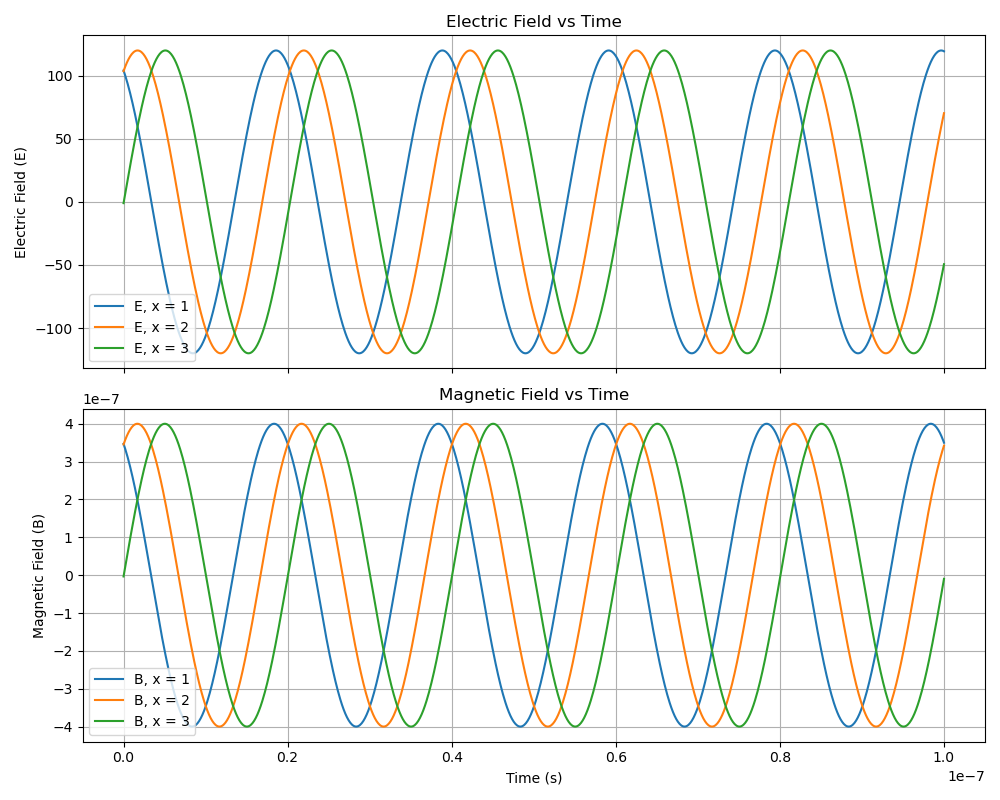
\includegraphics[width=1.05\columnwidth]{figs/Figure_1.png}
  \label{fig:fig1.12.8.8}

\end{figure}

\end{flushleft}

\end{document}
